\subsection{Glomerular Number Estimation}
In mammalian kidneys, \textit{nephrons} filter blood to form urine, and a network of capillaries called the \textit{glomerulus} found in the beginning of each nephron, performs the first step of this filtering. The variations in the number and size of glomeruli have been linked to several renal and systemic diseases \cite{brenner1988glomeruli, hoy2008nephron}. Though approaches such as acid maceration \cite{bonvalet1972compensatory} and the dissector/fractionator stereology technique \cite{bertram1992total} currently exist for measure the glomerular number and size, they require the destruction of the entire kidney. On the other hand, conventional histological methods determine the overall glomeruli statistics by extrapolating the measurements obtained from a few isolated sections. Consequently, these methods do not perform direct measurements and cannot localize the identified glomeruli to specific parts of the kidney. To address these challenges, the authors in \cite{beeman2011measuring} proposed a robust, non-destructive technique based on magnetic resonance imaging (MRI) to measure the number and size of glomeruli. This method accurately identifies the glomeruli by injecting cationic ferritin (CF), which causes a decrease in the MRI signal at the location of the glomeruli. The authors demonstrated that the glomerular counts obtained from the 3D MRI images were consistent with the standard histological procedures, while making the measurements in the entire kidney. A sample axial kidney image from 3-dimensional (3D) magnetic resonance imaging (MRI) data obtained for a CF-injected rat is shown in Figure \ref{Fig:samp}.

%\begin{figure}[t]
%\begin{minipage}[b]{1.0\linewidth}
%  \centering
%  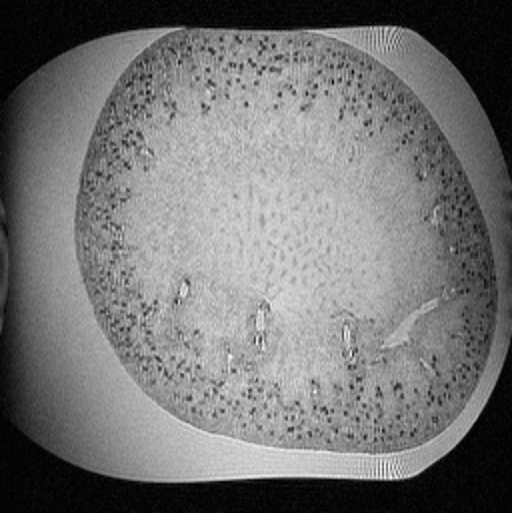
\includegraphics[width=4cm]{sample_kidney.png}
%\end{minipage}
%\caption{An example axial slice from the 3D MRI image obtained from a CF-injected rat. The MRI signal is comparatively weak at the locations of the glomerlus.}
%\label{Fig:samp}
%\end{figure} 

In this paper, we are interested in the estimation of the glomerular count from kidney MRI images. The problem of counting number of instances of an object in images (and videos) has been considered in the computer vision literature, and a number of approaches have been developed \cite{}. Several existing approaches are limited by their non-robustness to overlapping objects and noise, inability to provide accurate results when the objects are non-uniform, and need for time-consuming inference. Furthermore, approaches that avoid the hard problem of object detection, and take into account the spatial relationships between different local regions have been shown to provide superior results \cite{}. 

%\subsection{Our Approach}
%A typical solution to solving this problem is to apply a segmentation algorithm over the slices to identify isolated glomeruli, and subsequently count the number of connected regions. In this paper, we consider each $2-$D axial slice separately to obtain the glomerular count. As it can be observed in Figure \ref{Fig:samp}, each glomerulus occurs in the neighborhood of other glomeruli regions. Hence, segmentation approaches that take into account the neighborhood relations can be very effective in identifying the glomeruli. In particular, graph-embedding methods provide a principled framework to encode neighborhood information for each data sample. Though pixel-wise segmentation can be carried, robust estimation can be performed by using small patches. From our experiments, we found that image patches of size $5 \times 5$ provided the best results. In general, the problem of image segmentation is unsupervised, i.e., no training data is used to guide the segmentation process. However, by incorporating supervisory information from a user-generated training dataset, discriminative graphs can be constructed for learning a more efficient embedding. The user-generated training data, also referred to as the ground truth data, can be typically obtained by manually marking the glomerular regions in a few example images. Since the size, shape and form of glomeruli are similar across all kidneys in a species, any set of images can be chosen and marked by the user, irrespective of the particular subject under consideration. The other important challenge with unsupervised segmentation is its computational complexity. By learning a suitable discriminative model from labeled training data, the complexity of segmenting a test image can be reduced significantly, in addition to producing accurate results.
%
%In general, discriminative graph embedding approaches such as the linear discriminant analysis \cite{}, and the local discriminant embedding \cite{} work with graphs constructed based on locality. However, the performance of such locality-based graphs can be affected by factors such as (a) lack of robustness to noise, (b) non-uniform distribution of samples in the feature space, and (c) non-suitability of the locality assumption. To address these challenges, non-local graphs have been adopted by researchers in the recent years. In particular, $\ell_1$ graphs constructed based on sparse coding of data samples have been found to be very effective \cite{}. On the downside, such graphs are unsupervised, and computationally very intensive when compared to simple nearest-neighbor based graph construction techniques.
%
%In this paper, we propose to incorporate label information in $\ell_1$ graphs and obtain discriminative embeddings for patches from the kidney MRI images. Though our formulation is for a $2-$class case, this can be generalized to multi-class problems as well. The proposed method allows us to incorporate prior knowledge from the expert-marked ground truth images. Since discriminative projection directions are obtained from the training data, for test data, embeddings can be obtained by just extracting the patches and projecting them on to the discriminative directions, without the need for computing any graphs. As a result, the process of identifying the glomeruli regions and subsequently obtaining the count is computationally efficient, and provides improved results when compared to locality based graphs. We evaluate the proposed method using real data obtained using experiments with $5$ different rats \cite{}, and present comparisons to other conventional approaches such as stereology and acid maceration.